\documentclass[12pt]{article}

\usepackage{sbc-template}
\usepackage{graphicx,url}
%\usepackage[brazil]{babel}   
\usepackage[utf8]{inputenc}  
\usepackage{hyperref}
% \usepackage[T1]{fontenc}
% \usepackage{url}
% \usepackage{amsmath,amssymb}
% \usepackage{times}
% \usepackage{geometry}
% \usepackage{authblk}
% \usepackage{titlesec}
\usepackage{listings}
     
\sloppy

\lstset{
  basicstyle=\ttfamily\small,
  breaklines=true,
  columns=fullflexible
}

\title{
    Credit Card Customer: \\
    Descoberta de Subgrupos Utilizando Beam-Search
}

\author{
  Amanda Mendes Pinho\inst{1}\\
  Gabriel Tonioni Duarte\inst{2}\\
  João Vítor Fernandes Dias\inst{2}\\
  Larissa Duarte Santana\inst{2}
}

\address{
  Programa de Pós-Graduação em Engenharia Elétrica (PPGEE)\\
  \and
  Departamento de Ciência da Computação (DCC)\\
  Universidade Federal de Minas Gerais (UFMG)\\
    \email{mel2025@ufmg.br, {gabriel.tonioni, joaovitorfd2000, larissa.santana}@dcc.ufmg.br}

}
  
\begin{document}

\maketitle

\hspace{0.2em}

\begin{abstract}
    This study applies concepts of Descriptive Learning using the Beam Search algorithm to discover interpretable subgroups in a dataset containing behavioral variables of credit card customers. The dataset, available on Kaggle, includes anonymized information from approximately 9,000 users over a six-month period. The analysis enabled the identification of distinct customer profiles based on usage frequency, purchasing patterns, and financial behavior, demonstrating the effectiveness of Beam Search in identifying relevant patterns sensitive to search and evaluation parameters.
\end{abstract}

\begin{resumo}
    Este artigo aplica conceitos de Aprendizado Descritivo utilizando o algoritmo Beam Search para descoberta de subgrupos interpretáveis em um dataset com variáveis comportamentais de clientes de cartão de crédito. O conjunto de dados, disponível no Kaggle, contém informações anonimizadas de cerca de 9000 usuários em um período de 6 meses. A análise permitiu a identificação de perfis distintos de clientes com base na frequência de uso, padrão de compras e comportamento financeiro, demonstrando a eficácia do Beam Search na identificação de padrões relevantes sensíveis aos parâmetros de busca e avaliação.
\end{resumo}

\section{Introdução}

O aumento exponencial na geração de dados em diversas áreas tem impulsionado a busca por métodos avançados de análise capazes de extrair insights relevantes de forma eficiente, interpretável e útil para a tomada de decisão. Nesse contexto, técnicas de mineração de dados descritiva têm ganhado destaque por sua capacidade de revelar padrões e estruturas complexas em grandes volumes de dados, especialmente por meio da tarefa de descoberta de subgrupos, voltada à identificação de padrões locais que se destacam em relação a uma variável de interesse. Segundo \cite{proenca_22}, essa técnica apresenta vantagens robustas frente a ruídos e variações estatísticas, sendo particularmente adequada para domínios nos quais a interpretabilidade dos resultados e a consistência das descobertas são essenciais, como na medicina, no marketing e nas ciências sociais.

Conceitualmente, a descoberta de subgrupos ocupa uma posição intermediária entre abordagens puramente descritivas, como a análise exploratória de dados e as regras de associação, e métodos preditivos baseados em modelos supervisionados de classificação. Seu objetivo principal é identificar, dentro de uma população, subconjuntos que apresentem padrões estatisticamente relevantes com relação a uma variável-alvo, ou seja, grupos cuja distribuição difere de maneira significativa da distribuição global observada nos dados. Como apresentado por \cite{gamberger:02}, a tarefa visa gerar descrições compreensíveis e acionáveis desses segmentos, contribuindo para a explicação de fenômenos complexos e para o apoio à tomada de decisão em ambientes que exigem interpretação humana qualificada.

No setor financeiro, essa técnica adquire papel estratégico, dada a complexidade e sensibilidade dos dados envolvidos. A possibilidade de isolar perfis específicos de clientes ou comportamentos atípicos torna essa abordagem particularmente útil para aplicações como análise de crédito, detecção de fraudes e segmentação de consumidores. Ao possibilitar a geração de regras compreensíveis e orientadas por dados, a técnica viabiliza decisões mais informadas e direcionadas por parte das instituições financeiras. A literatura respalda a efetividade dessa estratégia em contextos aplicados: \cite{herrera:10} destaca sua importância em cenários que demandam transparência e clareza interpretativa, enquanto \cite{atzmueller:15} enfatiza o papel do algoritmo \textit{Beam Search} como uma estratégia eficaz para a exploração de espaços de busca de alta dimensionalidade. Tal abordagem tem se mostrado capaz de extrair subgrupos descritivos com elevado potencial explicativo, mesmo diante de conjuntos de dados complexos e heterogêneos.

Diversos estudos têm demonstrado o potencial da descoberta de subgrupos em contextos financeiros, seja para análise de comportamento de clientes ou para garantir a equidade e interpretabilidade de modelos preditivos. Por exemplo, \cite{maina:19} exploraram como subgrupos relevantes são preservados após processos de anonimização de dados financeiros, evidenciando a importância de manter estruturas interpretáveis mesmo em cenários de privacidade. Já \cite{dubowski:21} utilizaram técnicas de descoberta de subgrupos para identificar vieses e potenciais danos preditivos em sistemas de pontuação de risco, com foco em grupos vulneráveis dentro de bases financeiras.

Revisões mais amplas, como a de \cite{helal:16}, destacam casos práticos do uso de descoberta de subgrupos em finanças, reforçando seu papel como ferramenta analítica robusta. Ainda, \cite{herrera:10} discutem amplamente sua aplicação em marketing e comportamento do consumidor, áreas intrinsecamente ligadas às estratégias financeiras de segmentação, análise de crédito e fidelização.

Neste estudo, empregou-se uma base de dados do domínio financeiro em conjunto com o algoritmo SD, proposto por \cite{gamberger:02}, o qual adota a estratégia heurística de busca em feixe (\textit{Beam Search}) para a construção iterativa de regras descritivas. A técnica gera subgrupos por meio de uma função de qualidade parametrizada pela fórmula $q_g = \frac{TP}{FP + g}$, em que $TP$ e $FP$ representam, respectivamente, os verdadeiros e falsos positivos, e $g$ é um parâmetro de generalização ajustável. Essa metodologia demonstrou-se eficaz na identificação de perfis de comportamento entre clientes de cartão de crédito, revelando padrões associados à frequência de uso, volume de compras e níveis de endividamento.

\section{Metodologia}

O projeto foi desenvolvido sobre a base de dados \href{https://www.kaggle.com/datasets/arjunbhasin2013/ccdata/data}{\textit{Credit Card Dataset for Clustering}}, disponível no Kaggle. E para os experimentos realizados, foi utilizado o algoritmo Beam Search, implementado pela biblioteca Pysubgroup, que facilita a tarefa de descoberta de subgrupos ao fornecer métodos e ferramentas de implementação.

\subsection{Entendimento da Base de Dados}

O conjunto de dados resume o comportamento de uso de cerca de 9.000 titulares ativos de cartão de crédito num período de 6 meses. O arquivo está no nível do cliente, com 18 variáveis comportamentais. O que permite analisar perfis comportamentais de clientes, tais como clientes mais ou menos endividados (\texttt{BALANCE}, \texttt{CASH\_ADVANCE}), padrões de consumo (\texttt{PURCHASES}, \texttt{PURCHASES\_FREQUENCY}), capacidade de pagamento e uso do limite (\texttt{PAYMENTS}, \texttt{CREDIT\_LIMIT}), perfis de risco ou fidelização (\texttt{TENURE}, frequência de uso), oferecendo um contexto real sobre os dados dos clientes, o que permite a extração de insights relevantes em estudos de segmentação e comportamento financeiro.

Abaixo estão listadas todas as variáveis presentes nos dados, com uma explicação simples sobre o que representam:

\subsubsection{Variáveis de Saldo e Limite}
\begin{itemize}
    \item BALANCE (Saldo atual): Valor total restante na conta do cliente, disponível para compras.
    \item BALANCE\_FREQUENCY (Frequência de atualização do saldo): Valores próximos de 1 indicam atualização constante; próximo de 0, atualização esporádica.
    \item CREDIT\_LIMIT (Limite de crédito): Valor máximo de crédito que o cliente possui no cartão.
\end{itemize}

\subsubsection{Variáveis de Compras}
\begin{itemize}
    \item PURCHASES (Valor total de compras): Soma de todas as compras realizadas.
    \item ONEOFF\_PURCHASES (Compras únicas): Compras feitas de uma só vez (à vista ou em parcela única).
    \item INSTALLMENTS\_PURCHASES (Compras parceladas): Valor total de compras realizadas em parcelas.
    \item PURCHASES\_FREQUENCY (Frequência de compras): 1 indica compras muito frequentes, 0 indica compras raras.
    \item ONEOFFPURCHASESFREQUENCY (Frequência de compras únicas): 1 indica alta frequência de compras únicas; 0, baixa frequência.
    \item PURCHASESINSTALLMENTSFREQUENCY (Frequência de compras parceladas): 1 indica alta frequência de parcelamentos.
    \item PURCHASES\_TRX (Número de transações de compra): Quantidade total de compras feitas.
\end{itemize}

\subsubsection{Variáveis de Adiantamento de Dinheiro}
\begin{itemize}
    \item CASH\_ADVANCE (Valor de adiantamentos): Valor total de dinheiro adiantado (saques) pelo cliente.
    \item CASHADVANCEFREQUENCY (Frequência de adiantamentos): Frequência com que o cliente solicita adiantamentos.
    \item CASHADVANCETRX (Número de transações de adiantamento): Quantidade de vezes que o cliente realizou adiantamentos.
\end{itemize}

\subsubsection{Variáveis de Pagamento}
\begin{itemize}
    \item PAYMENTS (Valor total pago): Valor total pago pelo cliente.
    \item MINIMUM\_PAYMENTS (Pagamento mínimo): Valor mínimo que o cliente pagou em seus extratos.
    \item PRCFULLPAYMENT (Porcentagem de pagamento total): Porcentagem do valor total da fatura que foi paga. Valores próximos de 1 indicam pagamento completo frequente.
\end{itemize}

\subsubsection{Variáveis de Tempo de Relacionamento}
\begin{itemize}
    \item TENURE (Tempo de relacionamento): Tempo, em meses, que o cliente possui o cartão de crédito.
\end{itemize}

\subsection{Pré-Processamento de dados}

Antes da aplicação dos algoritmos de descoberta de subgrupos, foi necessário realizar etapas de pré-processamento dos dados, fundamentais para garantir a consistência e a qualidade das análises. Esse processo envolveu o tratamento de valores nulos e a discretização de variáveis numéricas, considerando as características específicas da base utilizada. As decisões adotadas nessa fase visaram mitigar o impacto de dados ausentes, adaptar a representação das variáveis ao contexto da análise e possibilitar a extração de padrões mais interpretáveis e estatisticamente relevantes nos experimentos subsequentes.

\subsubsection{Tratamento de Valores Nulos}

A base de dados apresentava alguns valores nulos, o que poderia comprometer a execução do algoritmo. Assim, adotaram-se duas estratégias distintas:
\begin{itemize}
    \item \textbf{Remoção de valores nulos}, utilizada no primeiro experimento;
    \item \textbf{Substituição pela mediana da coluna}, utilizada no segundo experimento, em razão da quantidade reduzida de dados ausentes.
\end{itemize}

\subsubsection{Discretização dos Dados}

A discretização é uma etapa importante no processo de descoberta de subgrupos, pois seletores categóricos geralmente tornam as regras mais interpretáveis para os analistas. Neste trabalho, foi utilizada a discretização por quartis (\texttt{qcut}) para transformar variáveis numéricas em categorias qualitativas. No entanto, nem todas as variáveis apresentaram uma distribuição apropriada para esse tipo de transformação. Para priorizar resultados mais imediatos e consistentes, apenas as colunas com número suficiente de valores distintos foram discretizadas. As demais foram mantidas em sua forma contínua, garantindo a preservação de suas propriedades numéricas para análise posterior.

O código abaixo ilustra o processo de discretização com tratamento de exceções para variáveis inadequadas:

\begin{lstlisting}[language=Python, caption={Discretização automática com quartis para variáveis numéricas.}]
df_binned = df.drop(columns=['CUST_ID'], errors='ignore')
df_binned = df.fillna(df.median(numeric_only=True))

numeric_cols = df_binned.select_dtypes(include=[np.number]).columns.tolist()

for col in numeric_cols:
    bin_col = f'{col}_BIN'
    try:
        df_binned[bin_col] = pd.qcut(df[col], q=4, labels=['low', 'med_low', 'med_high', 'high'])
    except ValueError:
        print(f"Skipping {col} - too few unique values to bin")
\end{lstlisting}

Durante o processo, as seguintes variáveis foram identificadas como inadequadas para discretização automática por apresentarem poucos valores únicos:

\begin{itemize}
    \item \texttt{BALANCE\_FREQUENCY}
    \item \texttt{ONEOFF\_PURCHASES}
    \item \texttt{INSTALLMENTS\_PURCHASES}
    \item \texttt{CASH\_ADVANCE}
    \item \texttt{ONEOFF\_PURCHASES\_FREQUENCY}
    \item \texttt{PURCHASES\_INSTALLMENTS\_FREQUENCY}
    \item \texttt{CASH\_ADVANCE\_FREQUENCY}
    \item \texttt{CASH\_ADVANCE\_TRX}
    \item \texttt{PRC\_FULL\_PAYMENT}
    \item \texttt{TENURE}
\end{itemize}

Dessa forma, foi possível aplicar a discretização apenas onde havia suporte estatístico, mantendo a integridade e a interpretabilidade dos dados ao longo das análises.

\subsection{Descoberta de Subgrupos com Beam Search}

A descoberta de subgrupos é uma tarefa descritiva voltada à identificação de subconjuntos de dados que se destacam em relação a uma variável-alvo, sendo especialmente útil em contextos que exigem interpretabilidade e personalização das regras extraídas. Nesse cenário, a biblioteca \texttt{pysubgroup} se destaca por oferecer uma estrutura flexível e eficiente para a definição de funções de qualidade, configuração das condições de descoberta e avaliação sistemática dos padrões gerados, apresentando compatibilidade com diferentes tipos de dados e objetivos analíticos \cite{lemmerich:18}. Entre os algoritmos disponíveis, o \textit{Beam Search} configura-se como uma estratégia heurística e controlada que visa encontrar subgrupos descritivos por meio de um processo composto por cinco etapas principais: \textbf{inicialização}, \textbf{expansão}, \textbf{avaliação}, \textbf{otimização (feixe)} e \textbf{iteração}.

Na fase de \textbf{inicialização}, o algoritmo parte de subgrupos simples, geralmente construídos a partir de descritores básicos. A \textbf{expansão} ocorre com o enriquecimento desses subgrupos por meio da adição de novos descritores, aumentando sua especificidade. Em seguida, a \textbf{avaliação} de cada subgrupo é realizada com base em uma função de qualidade, que define sua relevância conforme critérios estatísticos ou heurísticos previamente definidos. Durante a etapa de \textbf{seleção do feixe}, apenas os $k$ subgrupos com melhor desempenho são mantidos, garantindo que o algoritmo concentre esforços em regiões promissoras do espaço de busca. Por fim, a fase de \textbf{iteração} repete esse ciclo até que se atinja a profundidade máxima estabelecida ou os critérios de parada definidos sejam satisfeitos.

Portanto, no \textit{Beam Search}, os subgrupos gerados competem entre si por posições no feixe, sendo mantidos apenas aqueles com melhor desempenho de acordo com a função de qualidade. Isso garante uma busca eficiente por padrões relevantes e interpretáveis, mesmo em espaços de busca com múltiplos descritores.

\subsubsection{Configurações Experimentais}

Nesta etapa, foram definidos os principais parâmetros utilizados nos experimentos de descoberta de subgrupos. Como variáveis-alvo, selecionaram-se atributos diretamente relacionados ao comportamento de consumo dos clientes, a saber: \texttt{PURCHASES\_FREQUENCY}, \texttt{PURCHASES\_TRX}, \texttt{ONEOFF\_PURCHASES} e \texttt{BALANCE}. Essas variáveis foram escolhidas por refletirem aspectos relevantes da frequência de uso, volume de transações e situação financeira dos indivíduos analisados.

O espaço de busca foi explorado de duas maneiras: de forma completa, abrangendo todos os descritores disponíveis, e de forma segmentada, com restrições específicas para diferentes categorias de análise. Para a avaliação dos subgrupos gerados, foram empregadas distintas funções de qualidade, incluindo as medidas \texttt{stdQF} e \texttt{stdQFTscore}, bem como a métrica \texttt{WRAcc} (\textit{Weighted Relative Accuracy}). Esta última considera simultaneamente a precisão relativa do subgrupo e seu tamanho em relação ao conjunto total, o que permite equilibrar relevância estatística e representatividade \cite{vimieiro:24}.

As funções de qualidade utilizadas foram definidas conforme exemplificado no código da \autoref{lst:qualityfunc}, enquanto a criação das tarefas de busca foi realizada segundo o código ilustrado na \autoref{lst:task}.

\begin{lstlisting}[language=Python, caption={Função auxiliar para seleção da métrica de qualidade utilizada em cada experimento.}, label={lst:qualityfunc}]
def get_quality_function(name='stdQF', a=0.5, centroid='mean'):
    gen_quality_func = {
        'stdQF': ps.StandardQFNumeric(a, centroid=centroid),
        'stdQFTscore': ps.StandardQFNumericTscore(),
        'WRAcc': ps.WRAccQF(),
    }
    return gen_quality_func.get(name, gen_quality_func['stdQF'])
\end{lstlisting}

\begin{lstlisting}[language=Python, caption={Criação da tarefa de descoberta de subgrupos}]
def get_task(df, target, qf='stdQF', a=0.5, subgroup_size=10, desc_size=3):
    task = ps.SubgroupDiscoveryTask(
        df,
        targets[target],
        search_spaces[target],
        get_quality_function(qf, a),
        result_set_size=subgroup_size,
        depth=desc_size
    )
    return task
\end{lstlisting}

Adicionalmente, o parâmetro de recompensa por tamanho do subgrupo foi variado entre os valores 0.0, 0.3, 0.5 e 1.0, a fim de investigar o impacto do tamanho das regras na qualidade das descobertas. Também foram adotados valores fixos para as demais configurações experimentais, sendo definido o tamanho mínimo dos subgrupos como 10 instâncias, e o número máximo de descritores por subgrupo variando entre 3 e 8. Tais parâmetros impactam diretamente a complexidade das regras geradas, bem como a interpretabilidade dos padrões descobertos, especialmente em um contexto de análise comportamental com múltiplas variáveis interdependentes.

\subsubsection{Função de Avaliação Utilizada}

Nos experimentos envolvendo a variável-alvo \texttt{PURCHASES\_TRX}, buscou-se responder à pergunta: \textit{"quem utiliza muito o cartão de crédito?"}. Para isso, foi empregada uma função de avaliação baseada na diferença da média ponderada, definida conforme a seguinte equação:

\begin{equation}
    \text{score} = \alpha \times \text{instances}_{\text{subgroup}} \times (\text{mean}_{\text{sg}} - \text{mean}_{\text{dataset}})
\end{equation}

Nessa fórmula, o parâmetro $\alpha$ atua como um parâmetro de ajuste fino, permitindo controlar o equilíbrio entre a representatividade e a distinção dos subgrupos. Valores menores de $\alpha$ tendem a favorecer subgrupos mais compactos e diferenciados da média global, enquanto valores maiores priorizam a generalização e o tamanho dos grupos descobertos.

Para os experimentos com a variável-alvo \texttt{BALANCE}, a mesma função foi utilizada, com o objetivo de responder à pergunta: \textit{“qual o perfil de clientes mais endividados?”}. Dado que se trata também de um atributo numérico e contínuo, a função mostrou-se igualmente adequada, permitindo capturar subgrupos significativamente distintos em relação ao saldo devedor médio observado no conjunto de dados.

\section{Experimentos e Discussões}

Neste estudo, foram realizados dois tipos de experimentos distintos. O primeiro utilizou como variável-alvo o atributo \texttt{PURCHASES\_TRX}, com o objetivo principal de compreender o comportamento das variáveis ao se analisar descritores da área financeira, além de testar diferentes parâmetros das funções de qualidade. O segundo experimento teve como variável-alvo o atributo \texttt{BALANCE}, possuindo um caráter mais descritivo e interpretativo, voltado à análise dos padrões de consumo dos clientes.

\subsection{Análise do Atributo \texttt{PURCHASES\_TRX}}

O primeiro experimento teve como objetivo primário compreender os perfis de clientes que apresentam maior frequência de uso do cartão de crédito, e foi posteriormente direcionado à análise do impacto dos parâmetros da função de qualidade \texttt{StandardQFNumeric} sobre os subgrupos identificados pelo algoritmo \textit{Beam Search}.

\subsection{Análise de Padrões}

Ao analisar todos os experimentos, um perfil de cliente se destacou de forma consistente como o que mais utiliza o cartão: aquele que compra com alta frequência. Portanto, a característica preditiva com maior capacidade discriminativa em relação a um elevado número de transações (\texttt{PURCHASES\_TRX}) foi, inequivocamente, a frequência de compras (\texttt{PURCHASES\_FREQUENCY}). Clientes com \texttt{PURCHASES\_FREQUENCY} $\geq$ 1, ou seja, que realizam compras de forma consistente, apresentam uma média de 69 transações — um salto expressivo em relação à média global de 15 transações. Embora esse resultado seja esperado e relativamente evidente do ponto de vista interpretativo, ele reforça a validade da abordagem adotada, demonstrando que o algoritmo é capaz de identificar relações coerentes e alinhadas com o domínio do problema.

\subsection{Análise de Parâmetros}

A seguir, são apresentados os experimentos conduzidos com diferentes valores do parâmetro $\alpha$, evidenciando como essa variação permite refinar a análise e revelar nuances relevantes sobre este e outros perfis de clientes.

\subsubsection{Experimento 1}

Neste experimento, foi adotado o valor de $\alpha = 0{,}5$, o que direcionou o algoritmo a priorizar regras gerais, abrangendo uma quantidade expressiva de clientes.

\textbf{Regra principal:}
\begin{itemize}
    \item \texttt{PURCHASES\_FREQUENCY} $\geq$ 1
          \begin{itemize}
              \item Tamanho do subgrupo: 2.190 clientes
              \item Média de transações: 68{,}96
          \end{itemize}
\end{itemize}

\textbf{Insight:} A frequência de compras demonstrou ser a regra mais simples e, ao mesmo tempo, a mais preditiva para caracterizar clientes com elevado número de transações. Essa configuração se mostrou adequada para identificar os principais \textit{drivers} de comportamento presentes na base de dados.

\begin{figure}[h]
    \centering
    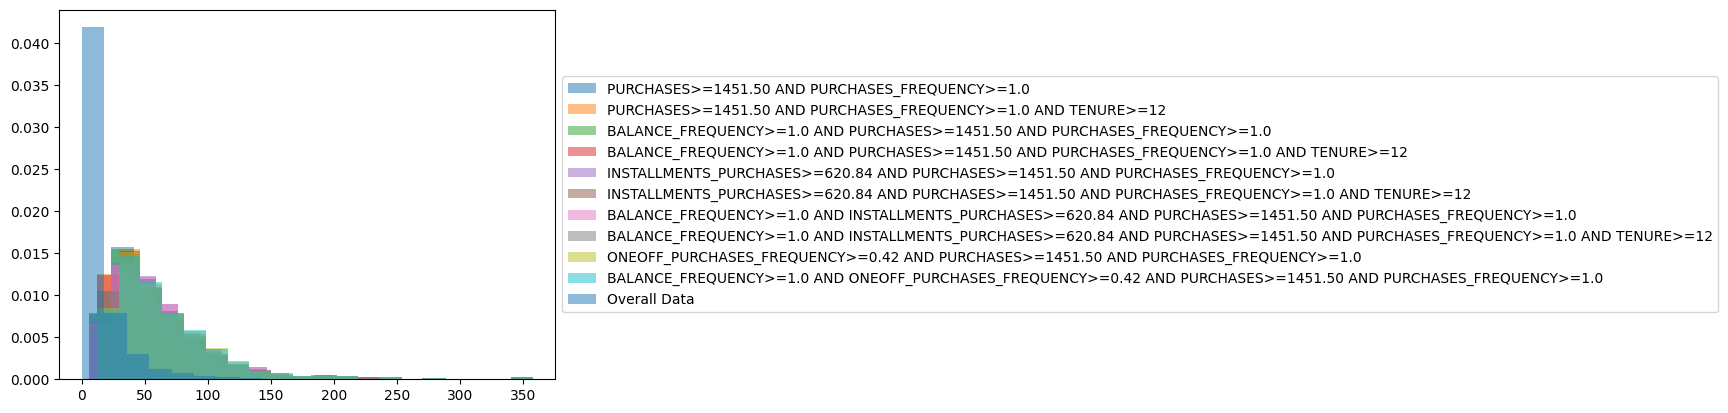
\includegraphics[width=1\textwidth]{imagens/experimento1.1.png}
    \caption{Distribuição de \texttt{PURCHASES\_TRX} no subgrupo definido por \texttt{PURCHASES\_FREQUENCY} $\geq$ 1. O experimento foi realizado com \texttt{depth} = 8, $\alpha$ = 0.5, e competição livre entre todos os seletores, resultando em subgrupos fortemente caracterizados pelo comportamento de compra.}
    \label{fig:experimento1_1}
\end{figure}

\begin{figure}[h]
    \centering
    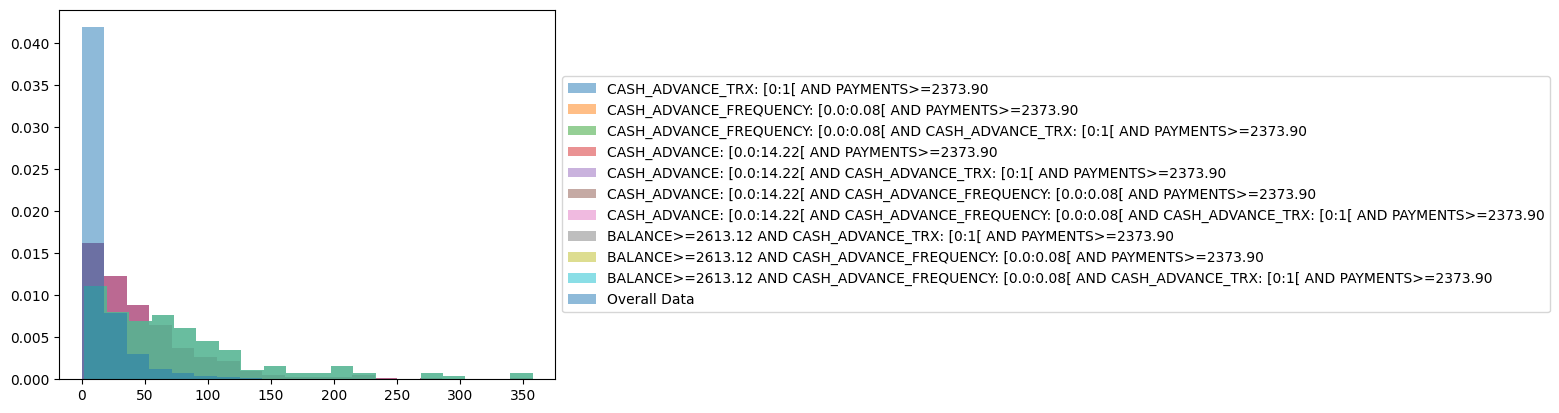
\includegraphics[width=1\textwidth]{imagens/experimento1.2.png}\caption{Distribuição de \texttt{PURCHASES\_TRX} no subgrupo definido por múltiplos descritores financeiros, com $\alpha = 0{,}3$, profundidade máxima igual a 8 e competição restrita a seletores do domínio financeiro. Observa-se que as descrições financeiras apresentam representatividade reduzida na composição do subgrupo.}\caption{Distribuição de \texttt{PURCHASES\_TRX} no subgrupo com múltiplos descritores e $\alpha = 0{,}3$}
    \label{fig:experimento2_1}
\end{figure}

\subsubsection{Experimento 2}

Neste experimento, foi utilizado o valor de $\alpha = 0{,}3$, o que alterou significativamente o comportamento do algoritmo. Com essa configuração, o \textit{Beam Search} passou a priorizar subgrupos menores e mais distintos da média global, favorecendo padrões mais extremos e específicos.

\textbf{Regra principal:}
\begin{itemize}
    \item \texttt{BALANCE\_FREQUENCY} $\geq$ 1.0 \\
          \texttt{INSTALLMENTS\_PURCHASES} $\geq$ 620.84 \\
          \texttt{ONEOFF\_PURCHASES} $\geq$ 834.8 \\
          \texttt{ONEOFF\_PURCHASE\_FREQUENCY} $\geq$ 0.42 \\
          \texttt{PAYMENTS} $\geq$ 2373.9
          \begin{itemize}
              \item Tamanho do subgrupo: 632 clientes
              \item Média de transações: 107{,}03
          \end{itemize}
\end{itemize}

\textbf{Insight:} Essa configuração revelou um perfil mais exclusivo de clientes que, além de apresentarem alta frequência de uso, também realizam transações de valores significativamente mais altos. O uso de $\alpha$ reduzido permitiu capturar nuances comportamentais mais específicas e distantes da média global, destacando subgrupos de maior valor transacional.

\begin{figure}[h]
    \centering
    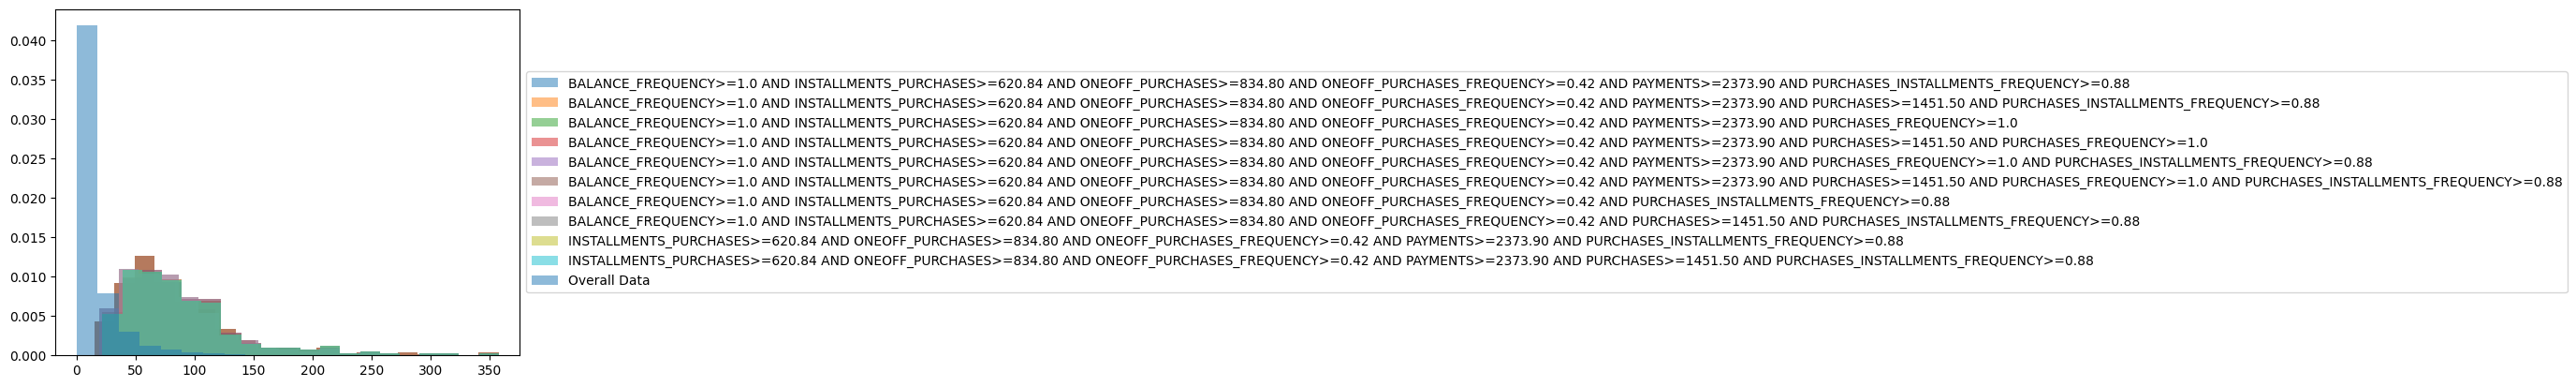
\includegraphics[width=1\textwidth]{imagens/experimento2.1.png}
    \caption{Distribuição de \texttt{PURCHASES\_TRX} no subgrupo com múltiplos descritores e $\alpha = 0{,}3$}
    \label{fig:experimento2_1}
\end{figure}
top-10  •  depth = 8  •  a = 0.3  •  competição entre todos os seletores
Subgrupos mais deslocados. Aqui aparecem  mais variáveis relacionadas à finanças.


\begin{figure}[h]
    \centering
    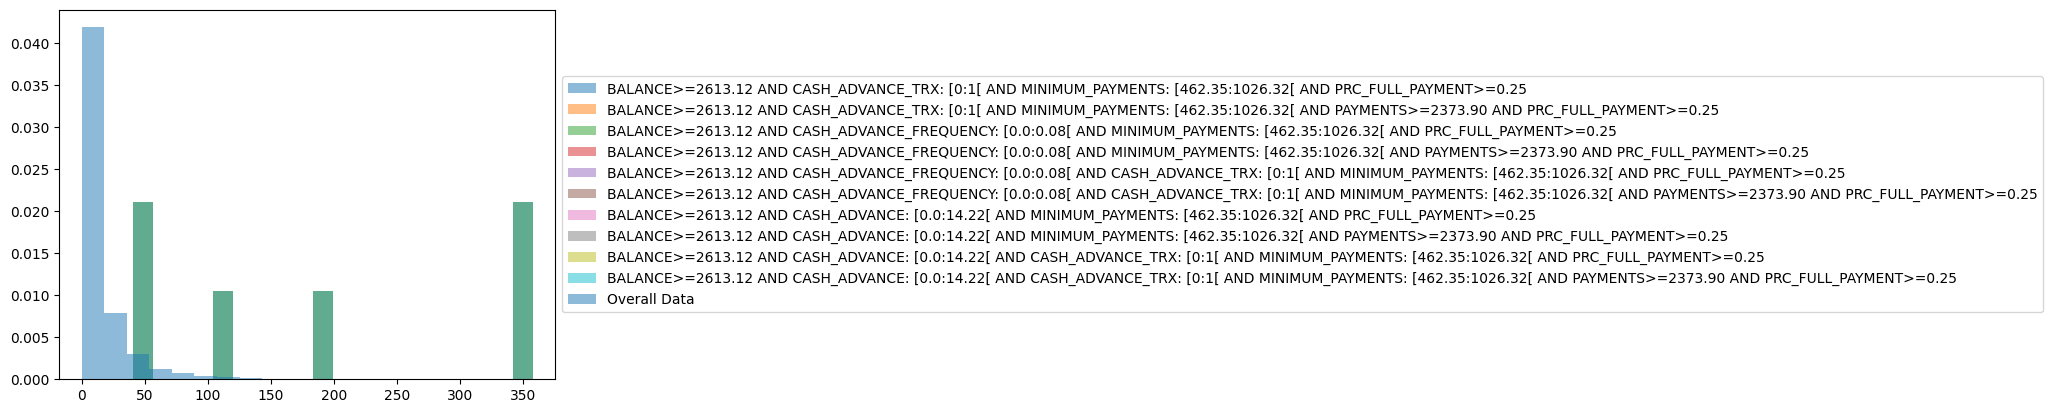
\includegraphics[width=1\textwidth]{imagens/experimento2.2.png}
    \caption{Distribuição de \texttt{PURCHASES\_TRX} no subgrupo com múltiplos descritores e $\alpha = 0{,}3$}
    \label{fig:experimento2_1}
\end{figure}
top-10  •  depth = 8  •  a = 0.3  •  apenas seletores de finanças
Diminuir o “a” nesse caso retorna subgrupos que chegam a cobrir apenas um usuário.


\subsubsection{Análise Crítica da Variação de $\alpha$}

O parâmetro $\alpha$ é um hiperparâmetro de ajuste fino que permite controlar o \textit{trade-off} entre encontrar subgrupos estatisticamente muito distintos (com grande diferença em relação à média global) e subgrupos que são representativos e acionáveis (com grande número de instâncias).

A escolha de valores para o expoente $\alpha$ próximos de 0{,}3 ou inferiores tende a degradar a qualidade geral dos subgrupos retornados, mas possibilita a exploração de relações entre variáveis menos fortemente correlacionadas com a variável-alvo. Isso pode ser útil para a indução de padrões menos óbvios. Embora padrões evidentes nem sempre sejam interessantes por si só, os descritores e as estatísticas associadas aos subgrupos ajudam a quantificar sua obviedade, o que pode ter utilidade prática em determinados contextos. Paralelamente, regras excessivamente grandes podem ser difíceis de interpretar e, em alguns casos, até redundantes. Para explorar de forma mais eficaz o espaço de seletores, pode ser vantajoso segmentá-los em diferentes categorias de análise e executar tarefas de descoberta de subgrupos separadamente. Portanto, não existe um valor universalmente ótimo para $\alpha$ — a escolha depende diretamente do objetivo final. Para uma visão geral dos principais perfis, $\alpha = 0{,}5$ se mostra uma combinação adequada. Já para identificar clientes \textit{premium} ou com comportamento mais extremo, $\alpha = 0{,}3$ tende a ser mais eficaz.

\subsection{Análise do Atributo \texttt{BALANCE}}

O segundo experimento possui um caráter mais descritivo e tem como objetivo principal identificar os tipos de clientes com comportamento mais impulsivo, que apresentam um saldo devedor acima da média global. O atributo \texttt{BALANCE} representa o saldo devedor, ou seja, o valor total que ainda precisa ser pago na fatura do cartão de crédito.

\begin{figure}[h]
    \centering
    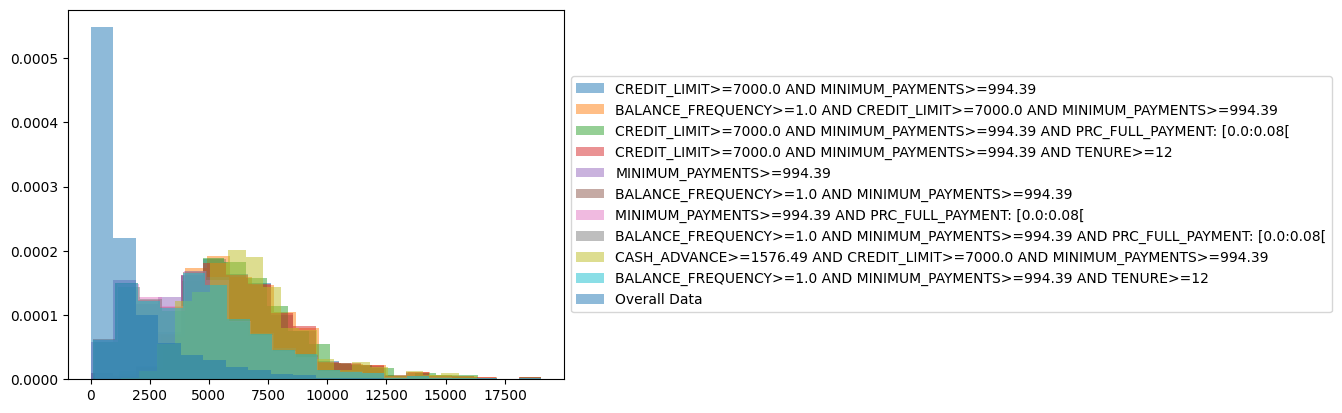
\includegraphics[width=1\textwidth]{imagens/experimento3.png}
    \caption{Distribuição do saldo devedor (\texttt{BALANCE}) para os subgrupos identificados com maior nível de endividamento, com destaque para os descritores \texttt{MINIMUM\_PAYMENTS}, \texttt{CREDIT\_LIMIT}, \texttt{PRC\_FULL\_PAYMENT} e \texttt{CASH\_ADVANCE}.}

    \label{fig:experimento2_1}
\end{figure}

De acordo com os resultados dos experimentos, as características que mais se repetem e definem os grupos com saldo devedor mais alto são descritas a seguir:

\begin{itemize}
    \item \textbf{Pagamento Mínimo Elevado}: A condição \texttt{MINIMUM\_PAYMENTS} $\geq$ 994.39 aparece em quase todas as regras de alta qualidade. Este é um indicativo direto de que o saldo devedor (\texttt{BALANCE}) é elevado, já que o pagamento mínimo geralmente é uma fração desse saldo. Trata-se do principal descritor encontrado, embora revele uma relação direta e esperada por conta da correlação entre as variáveis.

    \item \textbf{Limite de Crédito Alto}: A condição \texttt{CREDIT\_LIMIT} $\geq$ 7000.0 foi a segunda mais forte nos subgrupos identificados. Clientes com limites de crédito elevados tendem a acumular saldos devedores maiores.

    \item \textbf{Não Pagamento do Valor Total}: A condição \texttt{PRC\_FULL\_PAYMENT} $\in$ [0.0, 0.08[ indica que o cliente paga entre 0\% e 8\% da fatura, caracterizando o comportamento conhecido como "rotativo". Esses clientes financiam o saldo de um mês para o outro, acumulando juros e, por consequência, aumentando seu saldo devedor.

    \item \textbf{Frequência de Atualização do Saldo}: A condição \texttt{BALANCE\_FREQUENCY} $\geq$ 1.0 indica que o saldo desses clientes é atualizado com frequência, sugerindo que são usuários ativos do cartão.
\end{itemize}

Com base nesses resultados, foram identificados dois perfis distintos que definem a categoria de clientes com maior saldo devedor, descritos a seguir.

\subsubsection{O Saldo Mais Elevado}

O subgrupo com maior média de saldo devedor (R\$ 6.715,71) é caracterizado pela combinação das seguintes condições:
\begin{itemize}
    \item \texttt{CREDIT\_LIMIT} $\geq$ 7000.0
    \item \texttt{MINIMUM\_PAYMENTS} $\geq$ 994.39
    \item \texttt{CASH\_ADVANCE} $\geq$ 1576.49
\end{itemize}

Esse padrão sugere que o comportamento de realizar saques em dinheiro é um acelerador significativo do saldo devedor para clientes que já apresentam alto nível de endividamento.

\subsubsection{Clientes Antigos e Ativos}

Outro perfil recorrente nos subgrupos de maior \texttt{BALANCE} é o de clientes com:
\begin{itemize}
    \item \texttt{TENURE} $\geq$ 12
    \item \texttt{BALANCE\_FREQUENCY} $\geq$ 1.0
\end{itemize}

Esse comportamento indica que o endividamento tende a se consolidar ao longo do tempo, sendo mais comum entre clientes antigos e com uso contínuo do cartão.

Em resumo, a análise identificou com sucesso o perfil do cliente \textit{"endividado de alto valor"}: alguém com tempo de uso elevado, limite de crédito alto, que não quita a fatura mensal, utiliza crédito rotativo e realiza saques, comportamento esse que pode ser tratado como um padrão de risco elevado para instituições financeiras.

\section{Conclusão}

O mercado financeiro tem se tornado cada vez mais competitivo com o passar dos anos. Tratar todos os clientes da mesma forma torna-se, assim, uma oportunidade perdida para as empresas deste setor. Milhões de transações e dados de comportamento escondem padrões valiosos que as médias gerais não revelam. Dessa forma, utilizar a \textit{Descoberta de Subgrupos} neste contexto é ir além da análise superficial, buscando responder perguntas críticas de negócio de forma clara e direta. Ao encontrar grupos com regras compreensíveis, uma instituição financeira pode criar ações de marketing, gestão de risco e fidelização de forma cirurgicamente precisa, otimizando recursos e construindo um relacionamento mais inteligente e rentável com cada segmento de sua base de clientes.

Como resultado dos experimentos realizados, constatou-se que a manutenção dos atributos numéricos em sua forma contínua, por meio da não discretização dos dados, foi uma decisão assertiva, especialmente diante das características da base utilizada. Em um conjunto com número limitado de instâncias e atributos financeiros sensíveis, a discretização poderia comprometer a qualidade analítica, ao eliminar variações sutis, porém significativas, entre os registros — especialmente quando tais variações ocorrem em intervalos estreitos.

A preservação dos valores contínuos permitiu que os algoritmos identificassem padrões mais refinados, respeitando particularidades do comportamento financeiro dos clientes. Além disso, essa abordagem é relevante para funções de qualidade como a diferença da média ponderada, cujo desempenho depende diretamente da fidelidade dos valores numéricos originais.

A geração de insights significativos a partir dos subgrupos descobertos demonstrou depender fortemente da colaboração com especialistas da área financeira, pois embora os algoritmos possam identificar padrões estatisticamente relevantes, a validação semântica e a interpretação prática desses padrões requerem essa colaboração para a identificação de regras realmente úteis, em que é realizada a filtragem daquelas, que embora sejam interessantes estatisticamente, não seriam viáveis operacionalmente, por não refletirem comportamentos significativos no contexto da instituição.

\bibliography{referencias}
\bibliographystyle{sbc}

\end{document}